\documentclass[a4paper]{article}

% algumas packages para arrumar as tables co a margin:
% allows for temporary adjustment of side margins
\usepackage{changepage}
% provides filler text
\usepackage{lipsum}

% just makes the table prettier (see \toprule, \bottomrule, etc. commands below)
\usepackage{booktabs}


\usepackage[brazilian]{babel} %Para traduzir os textos
\usepackage[utf8]{inputenc} %Para poder usar acentos
\usepackage[a4paper]{geometry} %Para ajustar a parte geometrica da folha
\geometry{verbose,tmargin=2cm,bmargin=3cm,lmargin=3cm,rmargin=3cm} %Parte de margens
\setlength{\parindent}{0.5cm}
\usepackage{wrapfig} %Biblioteca Matematica/Grafica
\usepackage{mathptmx} %Biblioteca Matematica/Grafica
\renewcommand{\ttdefault}{mathptmx} %Biblioteca Matematica/Grafica
\usepackage{amsmath} %Biblioteca Matematica/Grafica
\usepackage{amssymb} %Biblioteca Matematica/Grafica
\usepackage[11pt]{moresize}% different letters sizes
\usepackage{float}% enables accurate location of tables
\usepackage{caption}% to make personalized captions
\usepackage{graphicx} %Para inclusão de imagens
\usepackage{indentfirst}
\usepackage{amsfonts}
\usepackage[T1]{fontenc}
%\usepackage[nottoc]{tocbibind}
\usepackage[framed,numbered]{mcode}
\graphicspath{ {images/} }

\makeatletter
\providecommand{\tabularnewline}{\\} %define

\title{Cálculo Computacional do Círculo de Mohr} % main title
\author{EM423 - Resistencia dos Materiais \\ \textsc{Grupo 13}}
\date{22 de Outubro, 2014}

\begin{document} % actually starts the document here
\maketitle

% members of the group
\begin{center}

	\begin{tabular}{l r l}
		Integrantes:\\\\
		 Felipe Tanios & RA: 155330  \\
		 Henrique Noronha Facioli & RA: 157986 \\
		 Kairo Vinicius & RA: 156075 \\
		 Lauro Souza e Cruz & RA: 156175\\
		 Mateus Coelho & RA: 156675 \\
	\end{tabular}
\end{center}


\newpage

\section{Introdução}


A força é uma ação que tende a alterar o estado do corpo,seja em repouso ou em movimento. É possível fazer o corpo acelerar, modificar a velocidade, a direção e o sentido de movimento. 
O estado do corpo submetido à ação de forças em torno de um ponto dentro do corpo material, é chamado de tensão. Força de tensão é uma força que quando aplicada a um corpo elástico, ele tende a se modificar, produzindo uma tensão. A representação desse estado de tensões é chamado de Círculo de Mohr.

Introduzido por  Christian Otto Mohr,  o Círculo de Mohr é uma forma gráfica bidimensional para resolver problemas de momentos de inércia, deformações e estado de tensões baseado na lei de transformação do tensor tensão de Cauchy. É possível usar o Círculo de Mohr somente quando cada plano for representado por um ponto em um sistema de coordenadas ($\sigma,\tau$).

O circulo de Mohr foi muito usado no passado quando não existiam calculadoras eletrônicas para obter graficamente e em escala, respostas para os problemas de distribuição de Tensões, porem atualmente ele é mais usado para visualizar completamente os estados de tensão em um ponto P considerado

\section{Resumo}

\section{Objetivo}
Prover uma interface de fácil utilização que, dadas as tensões de cisalhamento e as tensões normais em um plano, exibe em um gráfico personalizado o círculo de Mohr. O programa pode ser executado em múltiplas plataformas (Windows, Linux) e gera um log em formato de página de internet com os dados calculados. 

\section{Metodologia e Resultados}

\subsection{Metodologia}
Inicialmente buscamos um maior conhecimento do circulo de Mohr. Para isso utilizamos o livro texto indicado pelo professor e outro livro também da disciplina. Buscamos tambem outras fontes da propria universidade e bem como de outras universidades renomadas nacionais e internacionais para compreender o funcionamento do circulo e de todas as tensões e angulos apresentados por ele para uma melhor apresentação dos resultados ao usuario final.
Decidimos nomear os angulos como vimos nos slides de outros projetos de outros anos da disciplina, fornecidos pelo professor, exemplificado nas imagens abaixo:

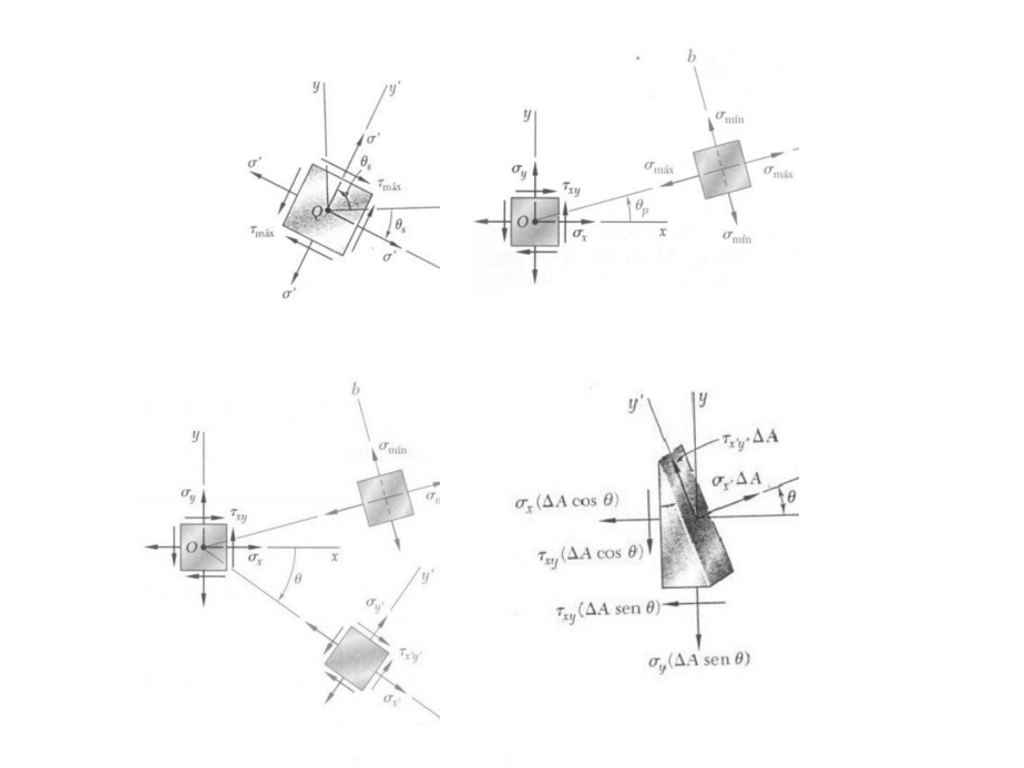
\includegraphics[scale = 0.4]{imagem1}



\subsection{Codigo}

\begin{lstlisting}
function run = run(self, tensao_x, tensao_y, tensao_cisalhamento, teta=0)
    sin = math.sin
    cos = math.cos
    rad = math.radians
    tensao_x = tensao_x
    tensao_y = tensao_y
    tensao_cisalhamento = tensao_cisalhamento
    teta = teta
    raio = 0
    % Tensao media (tau_med)
    tensao_principal_med = (tensao_x + tensao_y)/2.

    % Tensao media de Cisalhamento (tau_med)
    tensao_media_cisalhamento = (tensao_x - tensao_y)/2.

    % Raio do Circulo (R)
    raio = ((tensao_media_cisalhamento)**2  + 
                 (tensao_cisalhamento)**2)**0.5

    % Equilibrio das forcas nas direcao do Teta_sigma_x (sigma_x')
    tensao_x_linha = (tensao_principal_med + 
                           tensao_media_cisalhamento*cos(rad(2.*teta)) +
                           tensao_cisalhamento*sin(rad(2*teta)))

    % Equilibrio das forcas na direcao Teta_sigma_y (sigma_y')
    tensao_y_linha = (tensao_principal_med - 
                           tensao_media_cisalhamento*cos(2.*rad(teta)) -
                           tensao_cisalhamento*sin(2.*rad(teta)))

    % Equilibrio das forcas na direcao de Teta_tau (tau')
    tensao_cisalhamento_linha = -s elf.tensao_media_cisalhamento * 
                                        sin(2.*rad(teta))                     
                                        tensao_cisalhamento*cos(2.*rad(teta))

    % Tensao principal maxima (sigma_max)
    tensao_principal_max = tensao_principal_med + 
                                (((tensao_media_cisalhamento)**2) + 
                                tensao_cisalhamento**2)**0.5

    % Tensao principal minima (sigma_min)
    tensao_principal_min = tensao_principal_med - 
                            (((tensao_media_cisalhamento)**2) + 
                                tensao_cisalhamento**2)**0.5

    % Tensao de cisalhamento maxima (tau_max)
    tensao_cisalhamento_max = ((tensao_media_cisalhamento**2) + 
                                        tensao_cisalhamento**2)**0.5

    % Angulo entre os eixos sem rotacao ate o sigma minimo
    teta_p = ((math.degrees(math.atan((2.*tensao_cisalhamento) /
                                          (tensao_x-tensao_y))))/2.)
    % Angulo entre o eixo sem rotacao ate sigma_x'
    teta_s = ((math.degrees(math.atan(-(tensao_x-tensao_y) /
                                          (2.*tensao_cisalhamento))))/2.
\end{lstlisting}


\section{Formulas}

\begin{equation}
	\label{sigma_x'}
	\sigma_{x'} = \frac{\sigma_x + \sigma_y}{2} + \frac{\sigma_x - \sigma_y}{2}cos(2 \theta) + \tau_{xy}sen(2\theta)
\end{equation}

\begin{equation}
	\label{tau_xy'}	
	\tau_{x'y'} = -\frac{\sigma_x - \sigma_y}{2}sen(2 \theta) + \tau_{xy}cos(2\theta)
\end{equation}

\begin{equation}
	\label{sigma_y'}
	\sigma_{y'} = \frac{\sigma_x + \sigma_y}{2} - \frac{\sigma_x - \sigma_y}{2}cos(2 \theta) - \tau_{xy}sen(2\theta)
\end{equation}

\begin{equation}
	\sigma_x + \sigma_y = \sigma_{x'} + \sigma_{y'}
\end{equation}

\begin{equation}
	(\sigma_{x'} - \frac{\sigma_x + \sigma_y}{2})^2 + \tau_{x'y'}^2 = (\frac{\sigma_x - \sigma_y}{2})^2 + \tau_{xy}^2
\end{equation}

\begin{equation}
	\sigma_{med} = \frac{\sigma_x + \sigma_y}{2} 
\end{equation}

\begin{equation}
	R =  \sqrt{(\frac{\sigma_x - \sigma_y}{2})^2 + \tau_{xy}^2}  
\end{equation}

\begin{equation}
	tg(2\theta_p) = \frac{2\tau_xy}{\sigma_x - \sigma_y}
\end{equation}

\begin{equation}
	\sigma_{max} = \sigma{med} + R \therefore \sigma_{max} = \frac{\sigma_x + \sigma_y}{2} + \sqrt{(\frac{\sigma_x - \sigma_y}{2})^2 + \tau_{xy}^2}
\end{equation}

\begin{equation}
	\sigma_{max} = \sigma{med} + R
\end{equation}

\begin{equation}
	\tau_{max} = \sqrt{(\frac{\sigma_x - \sigma_y}{2})^2 + \tau_{xy}^2}
\end{equation}

\begin{equation}
	tg(2\theta_s) = - \frac{\sigma_x - \sigma_y}{2\tau_{xy}}
\end{equation}

\begin{equation}
	B = (\sigma_{x'}, \tau_{x'y'})
\end{equation}

\begin{equation}
	A = (\sigma_{y'}, -\tau_{x'y'})
\end{equation}


\section{Bibliografia}

\bibliography{mybib}


\end{document}
